%!TEX root = RBM.tex

\subsubsection{Annealed Importance Sampling\protect\footnote{Available at \protect\url{https://github.com/lzhbrian/MCMC/blob/ master/src/partition/AIS.m} in Matlab}}

\para{Algorithm} 
Annealed Importance Sampling(AIS)\cite{neal2001annealed,salakhutdinov2009learning} is probably one of the most preferable estimating methods avaible.

Previous work \cite{mackay2003information} have shown that if $P_{A}$ and $P_{B}$ in the SIS method is not close enough, the estimator would be very poor.

Based on SIS, the main idea of this algorithm is to gradually alter the value from an known $Z_{A}$ to our required $Z_{B}$ (or $Z_{K}$), by the following identity:
\begin{equation}
\frac{Z_{K}}{Z_{0}} = \frac{Z_{1}}{Z_{0}} \frac{Z_{2}}{Z_{1}} ... \frac{Z_{K}}{Z_{K-1}}
\end{equation}
where 
\begin{equation}
\frac{Z_{K}}{Z_{k+1}} = \frac{1}{M} \sum_{i=1}^{M} \frac{P_{k+1}^{*}(\mathbf x^{(i)})}{P_{k}^{*}(\mathbf x^{(i)})}
~~where~ x^{(i)} \sim P_{k}
\end{equation}
in which we can get $x_{k+1}$ from:
\begin{equation}
\begin{aligned}
p(h^{A}_{j}=1|\mathbf v) &= sigmoid\Bigg( (1-\beta_{k})\Bigg(\sum_{i}W^{A}_{ij}v_{i}+a^{A}_{j}\Bigg) \Bigg) \\
p(h^{B}_{j}=1|\mathbf v) &= sigmoid\Bigg( \beta_{k}\Bigg(\sum_{i}W^{B}_{ij}v_{i}+a^{B}_{j}\Bigg) \Bigg) \\ 
p(v'_{i}=1|\mathbf h) &= sigmoid\Bigg( (1-\beta_{k})\Bigg(\sum_{j}W^{A}_{ij}h_{i}^{A}+b^{A}_{i}\Bigg) \\
& + \beta_{k}\Bigg(\sum_{j}W^{B}_{ij}h_{j}^{B}+b^{B}_{i}\Bigg) \Bigg) 
\end{aligned}
\end{equation}
this procedure is shown in Figure~\ref{fig:xkxk1}.

\begin{figure}[tb]
% \vspace{-0.5in}
  	\centering
  	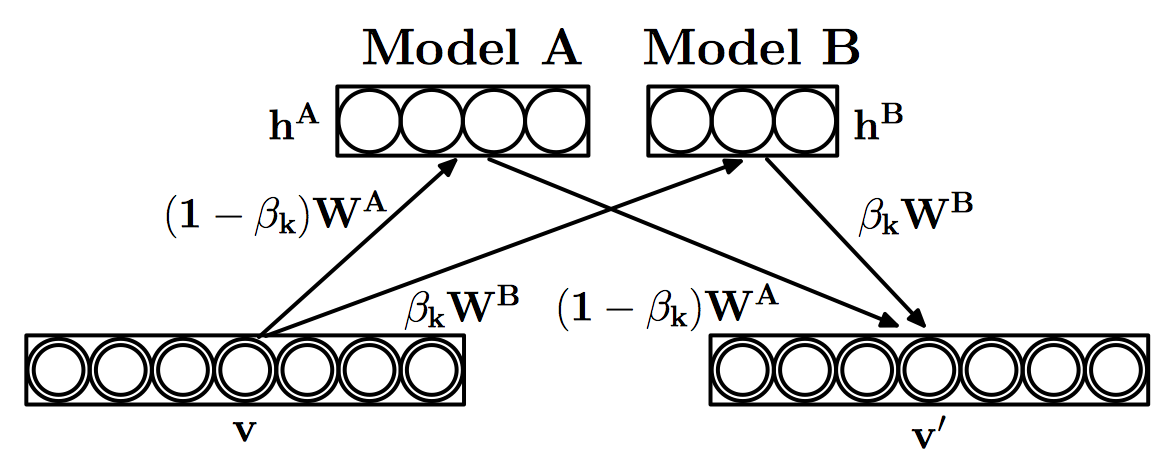
\includegraphics[width=0.4\textwidth]{figure/xkxk1.png}
% \vspace{-0.2in}
	\caption{The transition process from $x_{k}$ to $x_{k+1}$ which leaves $P_{k}(\mathbf v)$ invariant.}
	\label{fig:xkxk1}
\end{figure}

Note that model A indicates an initial model which we can easily compute all its configurations. Commonly, we choose an RBM model with $\theta = \{0,0,0\}$

$\mathbf \beta$ in the above equations is defined by users as a set of inverse temperatures $\{0= \beta_{1} < \beta_{2} < ... < \beta_{K} =1\}$, which can define a sequence of
\begin{equation}
P_{k}(\mathbf x) \propto P_{A}^{*}(\mathbf x)^{1-\beta_{k}} P_{B}^{*}(\mathbf x)^{\beta_{k}}
\end{equation}
where 
\begin{equation}
P^{*}_{k}(\mathbf v)=\sum_{h^{A}h^{B}}e^{(1-\beta_{k})E(\mathbf v, \mathbf h^{A};\theta_{A})+\beta_{k}E(\mathbf v,\mathbf h^{B};\theta_{B})}
\end{equation}


\para{Initialize $Z_{A}$ with dataset}
In \cite{salakhutdinov2009learning}, Ruslan also notice a method to make $Z_{A}$ near $Z_{B}$. As the length \& time limit, we will not specify the process here.

Originally, we initialize model A with a configuration of $\theta=\{0,0,0\}$. This method can use the training data to initialize the visible bias $\mathbf b$ to a desired value s.t. we can get a better outcome of the estimation.

In our real practice, we find that this method take less than 0.005 second to initialize $\mathbf b$ even for a very big model (i.e.784 visible and 500 hidden units), but have strongly improved the result as we will mention in the next subsection.


	\begin{algorithm}
        \caption{Annealed Importance Sampling}
        \begin{algorithmic}
        	\Require Required $\beta_{k}$ s.t. $0 = \beta_{0} < \beta_{1} < ... < \beta_{K} = 1$
        	\State Initialize $b_{A}$ by dataset
        	\State Sample $\mathbf x_{1}$ from $P_{A} = P_{0}$
            \For{$k = 1 \to K-1$}
                \State Sample $\mathbf x_{k+1}$ given $\mathbf x_{k}$ using $T_{k}(\mathbf x_{k+1} \longleftarrow \mathbf x_{k+1})$
			\EndFor
			\State Set $\omega_{AIS} = \prod_{k=1}^{K}P^{*}_{k}(\mathbf x_{k})/P^{*}_{k-1}(\mathbf x_{k})$
        \end{algorithmic}
    \end{algorithm}
